% =====================================================================
% Guía del estudiante -- Geometría 6° -- Trimestre I
% Hilo conductor: La geometría del fútbol
% Temas (propuesta de curriculo/plan-anual.md, sesiones 001-008):
%   angulos, angulosrectas, poligonos, triangulos
% Plan y ejercicios: guia-periodo-I-angulos-poligonos.plan.md
% Las clases citan los temas con \refguia{tema:...}. No borrar el .aux de esta guía.
% =====================================================================
% BORRADOR: el plan del trimestre está pendiente de aprobación de la docente (generación rápida 2026-09-14).
\documentclass[11pt]{article}
\makeatletter\def\input@path{{../../../../plantillas/estilo/}}\makeatother
\usepackage{mmcantillo}

% ======================== DATOS DE LA GUÍA ============================
\tipodocumento{Guía del estudiante}
\asignatura{Geometría}
\titulo{La geometría del fútbol: ángulos y polígonos}
\grado{6°}
\periodo{I}
\hiloconductor{La geometría del fútbol}
% ======================================================================
% DBA: matematicas grado 6 · DBA 5 — Propone y desarrolla estrategias de estimación, medición y
% cálculo de diferentes cantidades (ángulos, longitudes, áreas, volúmenes, etc.) para resolver
% problemas. · DBA 6 — Representa y construye formas bidimensionales y tridimensionales con el
% apoyo en instrumentos de medida apropiados. (DBA 4 en las construcciones con regla y compás.)
% (dba/matematicas/grados/grado06.tex)

\begin{document}

\encabezado

% ---------------------------------------------------------------------
% 1. Frase introductoria
% ---------------------------------------------------------------------
% verificado: https://www.claymath.org/library/annual_report/ar2008/08Interview.pdf — «The beauty of mathematics only shows itself to more patient followers» (Clay Mathematics Institute, Annual Report 2008, entrevista con M. Mirzakhani)
\frase{La belleza de las matemáticas solo se muestra a sus seguidores más pacientes.}
{Maryam Mirzakhani, entrevista del Clay Mathematics Institute (2008), trad. propia}

% ---------------------------------------------------------------------
% 2. Introducción
% ---------------------------------------------------------------------
\seccion{Introducción}

¿Desde dónde es más fácil hacer un gol? ¿Por qué las líneas de la cancha nunca se cruzan
donde no deben? ¿Por qué un balón hecho de piezas planas termina siendo redondo? Este
trimestre vamos a responder esas preguntas con geometría: midiendo y estimando
\textbf{ángulos}, estudiando las \textbf{rectas} que forman una cancha y descubriendo los
\textbf{polígonos} y los \textbf{triángulos} que se esconden en un balón.

Nuestro hilo conductor es \textbf{la geometría del fútbol}. En cada tema daremos un paso: del
ángulo de tiro de un delantero a las líneas de la cancha, de ahí a las piezas del balón y, al
final, a la razón por la que esas piezas se curvan hasta formar una esfera.

\textbf{Al terminar este trimestre podrás:}
\begin{itemize}
  \item clasificar ángulos, estimar su medida y medirlos con el transportador;
  \item reconocer rectas paralelas, perpendiculares y secantes, y calcular los ángulos que forman;
  \item identificar los elementos de un polígono y construir polígonos con regla y compás;
  \item clasificar y construir triángulos, y usar que sus ángulos suman $180^\circ$ para calcular
        ángulos de cualquier polígono.
\end{itemize}

Este trimestre trabaja dos Derechos Básicos de Aprendizaje del Ministerio de Educación
Nacional~\cite{mendba}:

\begin{dba}[Grado 6 · DBA 5]
Propone y desarrolla estrategias de estimación, medición y cálculo de diferentes cantidades
(ángulos, longitudes, áreas, volúmenes, etc.) para resolver problemas.
\end{dba}

\begin{dba}[Grado 6 · DBA 6]
Representa y construye formas bidimensionales y tridimensionales con el apoyo en instrumentos
de medida apropiados.
\end{dba}

% ---------------------------------------------------------------------
% 3. Marco teórico
% ---------------------------------------------------------------------
\seccion{Marco teórico}

\subsubsection*{Dar la vuelta en 360 partes}

Hacia el siglo V antes de nuestra era, los astrónomos de Babilonia dividían el camino que el
Sol parece recorrer en el cielo en 12 partes de 30, es decir, en 360 partes. De ahí viene la
costumbre de medir los ángulos en \textbf{grados}: una vuelta completa tiene $360^\circ$. No
dejaron escrito por qué eligieron 360. Se cree que influyeron su sistema de numeración, que
contaba de 60 en 60, y que el año tiene cerca de 360 días, pero es una suposición y no un hecho
comprobado~\cite{nrich,mactutorbab}.

\subsubsection*{Euclides pone nombres}

Hacia el año 300 antes de nuestra era, el griego Euclides escribió los \emph{Elementos}, un libro
que se usó para enseñar geometría durante más de dos mil años. Empieza con definiciones que
todavía usamos: un ángulo es \textbf{recto} cuando una recta que se levanta sobre otra forma
con ella dos ángulos iguales a lado y lado; es \textbf{obtuso} si es mayor que un recto y
\textbf{agudo} si es menor. Allí mismo clasificó los triángulos por sus lados (equilátero,
isósceles y escaleno) y por sus ángulos (rectángulo, obtusángulo y acutángulo). En la
proposición 32 de su primer libro demostró que los tres ángulos de cualquier triángulo suman
dos rectos, es decir, $180^\circ$~\cite{euclides}. Esa demostración la haremos en el tema 4.

\subsubsection*{Una cancha con reglas y un balón para la televisión}

Las medidas del fútbol las fija la IFAB en sus Reglas de Juego: el arco mide
$\qty{7,32}{m}$ entre los postes y $\qty{2,44}{m}$ de alto, el punto penal está a
$\qty{11}{m}$ del arco, y las líneas del área se trazan en ángulo recto con la línea de
meta~\cite{ifab}. Para el Mundial de México 1970 se fabricó el balón \emph{Telstar}: 32 piezas,
12 pentágonos negros y 20 hexágonos blancos, pensadas para que el balón se viera bien en los
televisores en blanco y negro de la época. Su nombre viene del inglés \emph{television star},
«estrella de la televisión»~\cite{adidas}. Desde entonces, ese dibujo es la imagen de un balón
de fútbol.

\subsubsection*{Maryam Mirzakhani: geometría de superficies curvas}

\textbf{Maryam Mirzakhani} nació en Teherán (Irán) en 1977. En 2014 se convirtió en la primera
mujer en recibir la Medalla Fields, el premio más importante para matemáticos jóvenes, por sus
estudios sobre la geometría de superficies curvas. Fue profesora de la Universidad de Stanford
y murió en 2017~\cite{mactutormirzakhani}. En la entrevista de la que viene la frase de esta
guía contó que en la escuela no le interesaban las matemáticas, y que su belleza se le mostró
poco a poco, con paciencia~\cite{clay2008}. Al final del trimestre veremos que el balón es,
justamente, una superficie curva armada con piezas planas.

% ---------------------------------------------------------------------
% 4. Temas
% ---------------------------------------------------------------------
\tema{Ángulos}\label{tema:angulos}

\begin{hilo}
Un delantero patea desde el punto penal y otro desde el borde del área. ¿Cuál tiene más
posibilidades de gol? Para decidirlo no basta con la distancia: hay que mirar qué tan
«abierto» ve cada uno el arco. Esa abertura es un ángulo.
\end{hilo}

\begin{definicion}[Ángulo]
Un \textbf{ángulo} está formado por dos rayos que salen del mismo punto, llamado
\textbf{vértice}. Los rayos son los \textbf{lados} del ángulo. Se escribe $\angle BAC$ (el
vértice va en el medio) o con una letra griega: $\alpha$, $\beta$, $\gamma$. Su medida indica
qué tan abiertos están sus lados y se da en \textbf{grados}: un grado ($1^\circ$) es la
$\frac{1}{360}$ parte de una vuelta completa. (Las definiciones de este trimestre siguen el
módulo de Geometría de las Guías de Apoyo~\cite{modulo}.)
\end{definicion}

Según su medida, los ángulos se clasifican así:

\begin{center}
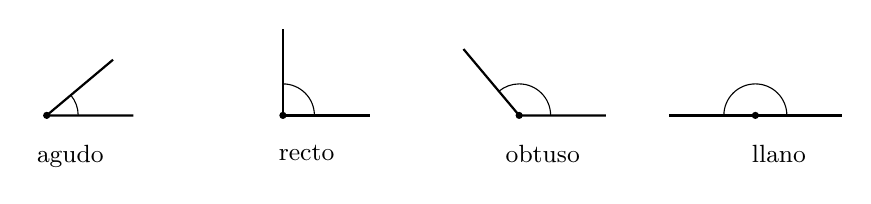
\begin{tikzpicture}[font=\small]
  \foreach \x/\a/\n in {0/40/agudo, 3/90/recto, 6/130/obtuso, 9/180/llano} {
    \begin{scope}[shift={(\x,0)}]
      \draw[thick] (1.1,0) -- (0,0) -- (\a:1.1);
      \draw (0.4,0) arc (0:\a:0.4);
      \fill (0,0) circle (1.3pt);
      \node[below] at (0.3,-0.25) {\n};
    \end{scope}}
\end{tikzpicture}
\end{center}

\begin{center}
\begin{tabular}{lll}
\textbf{Agudo}: menor que $90^\circ$ & \textbf{Recto}: $90^\circ$ & \textbf{Obtuso}: entre $90^\circ$ y $180^\circ$\\
\textbf{Llano}: $180^\circ$ & \textbf{Entrante}: entre $180^\circ$ y $360^\circ$ & \textbf{Completo}: $360^\circ$
\end{tabular}
\end{center}

\textbf{Medir con el transportador.} Se pone el centro del transportador sobre el vértice y la
línea del cero sobre uno de los lados; se lee el número por donde pasa el otro lado. Casi todos
los transportadores tienen dos escalas, una que empieza a la derecha y otra a la izquierda: hay
que leer la que empieza en el cero del lado que usamos. Por eso conviene \textbf{estimar antes de
medir}: si el ángulo se ve agudo y leemos $130^\circ$, leímos la escala equivocada y la medida
correcta es $180^\circ - 130^\circ = 50^\circ$.

\textbf{Estimar con referentes.} La esquina de un cuaderno es un ángulo recto. La mitad de esa
esquina es $45^\circ$ y un tercio, $30^\circ$. Comparando con esos referentes se puede estimar un
ángulo sin transportador y luego comprobarlo.

\begin{definicion}[Complementarios, suplementarios y conjugados]
Dos ángulos son \textbf{complementarios} si suman $90^\circ$, \textbf{suplementarios} si suman
$180^\circ$ y \textbf{conjugados} si suman $360^\circ$. Por ejemplo, el complemento de
$35^\circ$ es $55^\circ$, su suplemento es $145^\circ$ y su conjugado es $325^\circ$.
\end{definicion}

\begin{ejemplo}[El ángulo de tiro desde el punto penal]
Visto desde arriba, el arco es un segmento de $\qty{7,32}{m}$. El \textbf{ángulo de tiro} de un
jugador es el ángulo que tiene su vértice en el balón y sus lados hacia los dos postes. En el
dibujo, cada centímetro representa $\qty{4}{m}$. Desde el punto penal $A$, a $\qty{11}{m}$ del
centro del arco, ese ángulo mide cerca de $37^\circ$; desde el borde del área, $B$, a
$\qty{16,5}{m}$, mide cerca de $25^\circ$. El jugador que está más cerca y de frente ve el arco
más abierto.

\begin{center}
\begin{tikzpicture}[x=0.25cm, y=0.25cm, font=\small]
  \draw[gray] (-16,0) -- (16,0) node[right] {línea de meta};
  \draw[gray, dashed] (-20.16,0) -- (-20.16,16.5) -- (20.16,16.5) -- (20.16,0);
  \draw[line width=1.6pt] (-3.66,0) -- (3.66,0);
  \fill (-3.66,0) circle (4pt); \fill (3.66,0) circle (4pt);
  \coordinate (A) at (0,11); \coordinate (B) at (0,16.5);
  \draw (-3.66,0) -- (A) -- (3.66,0);
  \draw[dashed] (-3.66,0) -- (B) -- (3.66,0);
  \draw ([shift={(-108.4:3)}]A) arc (-108.4:-71.6:3);
  \fill (A) circle (4pt) node[left=2pt] {$A$};
  \fill (B) circle (4pt) node[above=2pt] {$B$};
  \node[below] at (0,-0.4) {arco ($\qty{7,32}{m}$)};
  \node[font=\footnotesize, right] at (20.4,8) {área grande};
\end{tikzpicture}
\end{center}
\end{ejemplo}

\begin{aplicacion}[Ángulos de tiro en el entrenamiento]
Los entrenadores ponen a practicar tiros desde puntos que ven el arco con distintos ángulos: de
frente, cerca, lejos y desde los lados. Cuando el ángulo de tiro es pequeño, basta un error de
pocos grados para que el balón salga por fuera del poste. Estimar ese ángulo a ojo, antes de
patear, es parte de la decisión del jugador.
\end{aplicacion}

\begin{preguntas}
\Needspace{8\baselineskip}
% Ejercicio: angulos-medicion-6-004 (nuevo: el banco no tenía ejercicios de estimar o medir ángulos)
\pregunta El arco mide $\qty{7,32}{m}$ entre los postes. Dibuja a escala ($\qty{1}{cm}$ por
metro) el arco y tres jugadores: $A$ en el punto penal, a $\qty{11}{m}$ del centro del arco;
$B$ en el borde del área, a $\qty{16,5}{m}$ del centro, de frente; $C$ a $\qty{11}{m}$ de la
línea de meta pero corrido $\qty{9}{m}$ hacia un lado. Primero estima el ángulo de tiro de cada
uno (el ángulo con vértice en el jugador y lados hacia los dos postes); luego mídelo con el
transportador. ¿Quién tiene más ángulo para hacer gol?
\espacio{5cm}
% Ejercicio: angulos-6-002
\pregunta Demuestra que si dos ángulos suplementarios son iguales, entonces cada uno es un
ángulo recto.
\renglones{3}
% Ejercicio: angulos-6-001
\pregunta Dos ángulos son conjugados si suman $360^\circ$. Demuestra que si dos ángulos tienen
el mismo conjugado, entonces son iguales.
\renglones{4}
\end{preguntas}

\begin{resumen}
\begin{itemize}
  \item Un ángulo son dos rayos con un vértice común; se mide en grados y una vuelta tiene $360^\circ$.
  \item Según su medida es agudo, recto, obtuso, llano, entrante o completo.
  \item Antes de medir con el transportador, estima: así descubres si leíste la escala equivocada.
  \item Complementarios suman $90^\circ$; suplementarios, $180^\circ$; conjugados, $360^\circ$.
\end{itemize}
\end{resumen}

% ---------------------------------------------------------------------
\tema{Ángulos entre rectas}\label{tema:angulosrectas}

\begin{hilo}
Una cancha de fútbol es un dibujo hecho con rectas. La línea de meta y la línea media nunca se
encuentran, por más larga que sea la cancha; la línea lateral y la de meta forman en cada
esquina un ángulo recto. Esas relaciones entre rectas tienen nombre.
\end{hilo}

\begin{definicion}[Posiciones de dos rectas en el plano]
Dos rectas del mismo plano son \textbf{paralelas} si no se cortan por más que se prolonguen
($l_1 \parallel l_2$); son \textbf{secantes} si se cortan en un punto; y son
\textbf{perpendiculares} si al cortarse forman cuatro ángulos rectos ($l_1 \perp l_2$). Las
secantes que no son perpendiculares se llaman \textbf{oblicuas}.
\end{definicion}

Cuando dos rectas se cortan forman cuatro ángulos. Dos de ellos que comparten el vértice y un
lado son \textbf{adyacentes}; como juntos forman un ángulo llano, suman $180^\circ$. Dos que no
comparten ningún lado se llaman \textbf{opuestos por el vértice}.

\begin{center}
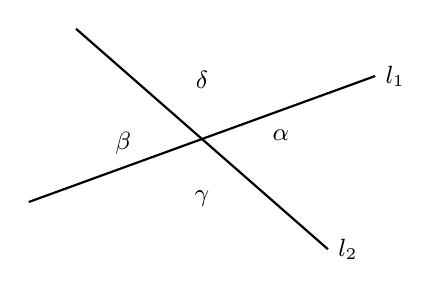
\begin{tikzpicture}[font=\small]
  \draw[thick] (-2.2,-0.8) -- (2.2,0.8) node[right] {$l_1$};
  \draw[thick] (-1.6,1.4) -- (1.6,-1.4) node[right] {$l_2$};
  \node at (1.0,0.05) {$\alpha$};
  \node at (0,0.75) {$\delta$};
  \node at (-1.0,-0.05) {$\beta$};
  \node at (0,-0.75) {$\gamma$};
\end{tikzpicture}
\end{center}

\begin{teorema}[Los ángulos opuestos por el vértice son iguales]
En el dibujo, $\alpha$ y $\delta$ son adyacentes, así que $\alpha + \delta = 180^\circ$. También
$\beta$ y $\delta$ son adyacentes: $\beta + \delta = 180^\circ$. Entonces
$\alpha + \delta = \beta + \delta$ y, quitando $\delta$ de los dos lados, $\alpha = \beta$.
\end{teorema}

La \textbf{bisectriz} de un ángulo es la recta que lo divide en dos ángulos iguales. Se traza
con compás: con centro en el vértice se marca un arco que corte los dos lados; desde esos dos
puntos, con la misma abertura, se trazan dos arcos que se cortan; la recta que une el vértice
con ese corte es la bisectriz.

\begin{aplicacion}[Las líneas de la cancha]
La IFAB exige que las líneas del área grande y del área chica se tracen en ángulo recto con la
línea de meta~\cite{ifab}. Así, la línea del área que queda frente al arco es paralela a la
línea de meta: dos rectas perpendiculares a una misma recta son paralelas entre sí. Quienes
pintan una cancha usan esa propiedad: trazan perpendiculares con una escuadra grande o con una
cuerda y obtienen líneas paralelas sin medir ángulos de nuevo.
\end{aplicacion}

\begin{preguntas}
% PENDIENTE: el banco no tiene ejercicios de ángulos adyacentes y opuestos por el vértice con
% medidas, ni de reconocer paralelas y perpendiculares (solo se agregan ejercicios del banco).
% Ejercicio: triangulos-6-003
\pregunta Indica si la afirmación es verdadera o falsa y argumenta tu respuesta (las figuras
están en un plano): «Las bisectrices de dos ángulos adyacentes son perpendiculares».
\renglones{4}
% Ejercicio: triangulos-6-005
\pregunta Indica si la afirmación es verdadera o falsa y argumenta tu respuesta (las figuras
están en un plano): «Las bisectrices de dos ángulos suplementarios adyacentes son
perpendiculares».
\renglones{4}
\end{preguntas}

\begin{resumen}
\begin{itemize}
  \item Paralelas: no se cortan. Secantes: se cortan en un punto. Perpendiculares: se cortan
        formando cuatro ángulos rectos.
  \item Los ángulos adyacentes que forman dos secantes suman $180^\circ$.
  \item Los ángulos opuestos por el vértice son iguales.
  \item La bisectriz divide un ángulo en dos iguales y se traza con compás.
\end{itemize}
\end{resumen}

% ---------------------------------------------------------------------
\tema{Polígonos}\label{tema:poligonos}

\begin{hilo}
Mira de cerca un balón clásico: no es una esfera lisa, sino 32 piezas planas cosidas. Cada
pieza es una figura cerrada con lados rectos: un polígono.
\end{hilo}

\begin{definicion}[Polígono]
Un \textbf{polígono} es una figura plana y cerrada formada por segmentos de recta, sus
\textbf{lados}, que se unen de dos en dos por sus extremos, los \textbf{vértices}. Un círculo o
una figura con un lado curvo no son polígonos. Una \textbf{diagonal} es un segmento que une dos
vértices que no son vecinos.
\end{definicion}

Los polígonos se nombran por su número de lados: triángulo (3), cuadrilátero (4), pentágono
(5), hexágono (6), heptágono (7), octágono (8), eneágono (9), decágono (10). Además, un polígono
es \textbf{equilátero} si tiene todos sus lados iguales, \textbf{equiángulo} si tiene todos sus
ángulos iguales y \textbf{regular} si es las dos cosas. Es \textbf{convexo} si ninguno de sus
ángulos internos es entrante, y \textbf{cóncavo} si alguno lo es.

\begin{ejemplo}[Contar diagonales]
Desde un vértice de un polígono de $n$ lados no se puede trazar diagonal ni a él mismo ni a sus
dos vecinos: salen $n - 3$ diagonales. Como hay $n$ vértices y cada diagonal se cuenta dos veces
(una desde cada extremo), el total es $\dfrac{n(n-3)}{2}$. En el hexágono: de cada vértice salen
3 diagonales y en total hay $\frac{6 \cdot 3}{2} = 9$.
\end{ejemplo}

\begin{ejemplo}[Construir un hexágono regular con compás]
Se traza una circunferencia y, \emph{sin cambiar la abertura del compás}, se apoya la punta en
un punto de ella y se marca otro punto; desde ese, el siguiente, y así seis veces: se vuelve al
punto de partida. Uniendo los seis puntos queda un hexágono regular. Funciona porque el
hexágono regular está formado por seis triángulos equiláteros con un vértice en el centro: su
lado mide lo mismo que el radio.

\begin{center}
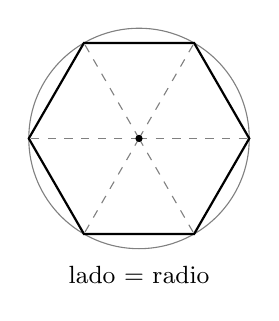
\begin{tikzpicture}[font=\small]
  \draw[gray] (0,0) circle (1.4);
  \draw[thick] (0:1.4) \foreach \a in {60,120,...,360} { -- (\a:1.4) } -- cycle;
  \foreach \a in {0,60,...,300} \draw[gray, dashed] (0,0) -- (\a:1.4);
  \fill (0,0) circle (1.3pt);
  \node[below] at (0,-1.5) {lado = radio};
\end{tikzpicture}
\end{center}
\end{ejemplo}

\begin{aplicacion}[El balón Telstar]
Las 32 piezas del Telstar son 12 pentágonos y 20 hexágonos regulares~\cite{adidas}. Todas las
piezas de cada tipo son iguales, para que se puedan coser en cualquier orden. Hoy los balones se
fabrican con otras formas de piezas, pero el dibujo de pentágonos y hexágonos sigue siendo el
que usamos para dibujar un balón.
\end{aplicacion}

\begin{preguntas}
\Needspace{8\baselineskip}
% Ejercicio: poligonos-6-001 (nuevo: el banco no tenía nada para este tema)
\pregunta Completa la tabla para el pentágono, el hexágono y el octágono.
\begin{center}
\renewcommand{\arraystretch}{1.4}
\begin{tabular}{|l|c|c|c|c|}\hline
Polígono & Lados & Vértices & Diagonales desde un vértice & Total de diagonales\\\hline
Pentágono & & & & \\\hline
Hexágono & & & & \\\hline
Octágono & & & & \\\hline
\end{tabular}
\end{center}
% Ejercicio: poligonos-6-005 (nuevo: el banco no tenía nada para este tema)
\pregunta El balón Telstar del Mundial de 1970 tenía 12 pentágonos y 20 hexágonos cosidos.
\begin{opciones*}(1)
  \item ¿Cuántos lados suman todas las piezas?
  \item Cada costura une el lado de una pieza con el lado de otra: ¿cuántas costuras tiene el balón?
  \item En cada vértice del balón se juntan tres piezas: ¿cuántos vértices tiene?
\end{opciones*}
\espacio{3.5cm}
\end{preguntas}

\begin{resumen}
\begin{itemize}
  \item Un polígono es una figura plana y cerrada de lados rectos; se nombra por su número de lados.
  \item Regular = todos los lados iguales y todos los ángulos iguales.
  \item De cada vértice salen $n - 3$ diagonales; en total hay $\frac{n(n-3)}{2}$.
  \item En el hexágono regular el lado mide lo mismo que el radio: se construye con compás.
\end{itemize}
\end{resumen}

% ---------------------------------------------------------------------
\tema{Triángulos}\label{tema:triangulos}

\begin{hilo}
El triángulo es el polígono con menos lados posible, y con triángulos se puede estudiar
cualquier otro polígono. Con ellos vamos a responder la pregunta del trimestre: ¿por qué 32
piezas planas terminan formando una esfera?
\end{hilo}

\begin{definicion}[Clasificación de los triángulos]
\textbf{Por sus lados:} equilátero (tres lados iguales), isósceles (dos lados iguales) y escaleno
(tres lados distintos). \textbf{Por sus ángulos:} acutángulo (tres ángulos agudos), rectángulo
(un ángulo recto) y obtusángulo (un ángulo obtuso). En todo triángulo, a lados iguales se
oponen ángulos iguales.
\end{definicion}

\textbf{Construir un triángulo con regla y compás.} Dados tres lados, se traza el primero con la
regla; con centro en un extremo y abertura igual al segundo lado se traza un arco, y con centro
en el otro extremo y abertura igual al tercero, otro arco. Donde se cortan está el tercer vértice.
Si los arcos no se cortan, el triángulo no existe.

\begin{teorema}[Desigualdad triangular]
En todo triángulo, cada lado es menor que la suma de los otros dos. Por eso con 3, 4 y
$\qty{8}{cm}$ no se puede construir un triángulo: $3 + 4 = 7 < 8$.
\end{teorema}

\Needspace{16\baselineskip}
\begin{teorema}[Los ángulos de un triángulo suman $180^\circ$]
Por el vértice $C$ del triángulo $ABC$ se traza la recta paralela al lado $AB$. Los ángulos
marcados con la misma letra son iguales (son ángulos alternos entre paralelas). Arriba, en $C$,
los tres ángulos $\alpha$, $\gamma$ y $\beta$ forman un ángulo llano: $\alpha + \beta + \gamma =
180^\circ$~\cite{euclides}.

\begin{center}
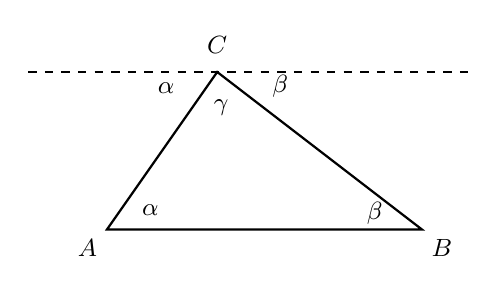
\begin{tikzpicture}[font=\small]
  \coordinate (A) at (0,0); \coordinate (B) at (4,0); \coordinate (C) at (1.4,2);
  \draw[thick] (A) -- (B) -- (C) -- cycle;
  \draw[dashed] (-1,2) -- (4.6,2);
  \node[below left] at (A) {$A$}; \node[below right] at (B) {$B$}; \node[above=3pt] at (C) {$C$};
  \node at (0.55,0.25) {$\alpha$}; \node at (3.4,0.2) {$\beta$}; \node at (1.45,1.55) {$\gamma$};
  \node at (0.75,1.8) {$\alpha$}; \node at (2.2,1.82) {$\beta$};
\end{tikzpicture}
\end{center}
\end{teorema}

Si se prolonga un lado, el \textbf{ángulo externo} que se forma es el suplemento del interno
que está a su lado, y es igual a la suma de los otros dos ángulos internos.

\subsubsection*{Del triángulo al polígono}

Desde un vértice de un polígono de $n$ lados salen $n - 3$ diagonales, que lo dividen en
$n - 2$ triángulos. Los ángulos de esos triángulos forman, juntos, los ángulos del polígono. Por
eso:
\[
  \text{suma de los ángulos internos de un polígono de } n \text{ lados} = 180^\circ\,(n - 2).
\]
En un polígono regular todos los ángulos son iguales, así que cada uno mide
$\dfrac{180^\circ (n-2)}{n}$.

\begin{center}
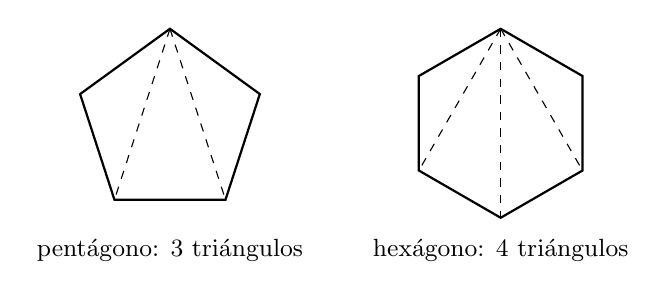
\begin{tikzpicture}[font=\small]
  \begin{scope}
    \draw[thick] (90:1.2) \foreach \a in {162,234,306,18} { -- (\a:1.2) } -- cycle;
    \draw[dashed] (90:1.2) -- (234:1.2); \draw[dashed] (90:1.2) -- (306:1.2);
    \node[below] at (0,-1.35) {pentágono: 3 triángulos};
  \end{scope}
  \begin{scope}[shift={(4.2,0)}]
    \draw[thick] (90:1.2) \foreach \a in {150,210,...,390} { -- (\a:1.2) } -- cycle;
    \foreach \a in {210,270,330} \draw[dashed] (90:1.2) -- (\a:1.2);
    \node[below] at (0,-1.35) {hexágono: 4 triángulos};
  \end{scope}
\end{tikzpicture}
\end{center}

\begin{ejemplo}[Un piso de hexágonos]
Cada ángulo del hexágono regular mide $\frac{180^\circ \cdot 4}{6} = 120^\circ$. Tres hexágonos
alrededor de un punto suman $3 \cdot 120^\circ = 360^\circ$: completan el giro y quedan planos,
como las celdas de un panal. Con pentágonos regulares ($108^\circ$) no se puede: tres suman
$324^\circ$ y cuatro se pasan. Los únicos polígonos regulares que cubren solos un piso son el
triángulo equilátero, el cuadrado y el hexágono.

\begin{center}
\begin{tikzpicture}[scale=0.7]
  \foreach \c in {90,210,330} {
    \draw[thick] ($(\c:1)+(\c+180:1)$) \foreach \k in {1,...,5} { -- ($(\c:1)+(\c+180+60*\k:1)$) } -- cycle;
  }
  \fill (0,0) circle (2pt);
\end{tikzpicture}
\end{center}
\end{ejemplo}

\begin{aplicacion}[Por qué el balón es redondo]
En cada vértice del Telstar se juntan un pentágono y dos hexágonos. Si quisiéramos ponerlos
planos sobre una mesa, sus ángulos no alcanzarían a completar la vuelta alrededor del vértice:
quedaría un pequeño hueco. Al coser los bordes para cerrar ese hueco, las piezas se levantan un
poco. Repetido en todos los vértices, el conjunto se cierra en una esfera. Los tres ángulos
que se juntan en cada vértice suman $108^\circ + 120^\circ + 120^\circ = 348^\circ$: les faltan
$12^\circ$ para completar la vuelta.
\end{aplicacion}

\begin{preguntas}
% Ejercicio: triangulos-6-001
\pregunta Indica si la afirmación es verdadera o falsa y argumenta tu respuesta: «La suma de
las longitudes de dos lados de un triángulo puede ser mayor que el tercer lado».
\renglones{3}
\Needspace{10\baselineskip}
% Ejercicio: triangulos-6-013, triangulos-6-014
\pregunta Indica si cada afirmación es verdadera o falsa y argumenta tu respuesta:
\begin{opciones*}(1)
  \item «Ningún triángulo puede tener más de un ángulo recto».
  \item «Ningún triángulo puede tener más de un ángulo obtuso».
\end{opciones*}
\renglones{4}
% Ejercicio: triangulos-6-015
\pregunta Los ángulos agudos de un triángulo rectángulo son tales que uno es el doble del otro.
¿Cuánto miden los tres ángulos internos?
\espacio{2.5cm}
% Ejercicio: triangulos-6-017
\pregunta El ángulo opuesto a la base de un triángulo isósceles mide $50^\circ$. ¿Cuánto miden
los otros dos ángulos internos?
\espacio{2.5cm}
% Ejercicio: triangulos-6-020
\pregunta En el triángulo $ABC$, el ángulo con vértice en $A$ mide $30^\circ$ y el ángulo
externo en $B$ mide $110^\circ$. ¿Cuánto mide el ángulo $C$?
\espacio{2.5cm}
\end{preguntas}

\begin{resumen}
\begin{itemize}
  \item Por sus lados: equilátero, isósceles, escaleno. Por sus ángulos: acutángulo,
        rectángulo, obtusángulo.
  \item Cada lado es menor que la suma de los otros dos (desigualdad triangular).
  \item Los ángulos internos de un triángulo suman $180^\circ$; los de un polígono de $n$ lados,
        $180^\circ (n - 2)$.
  \item Un piso se cubre con un solo polígono regular si sus ángulos completan $360^\circ$
        alrededor de un punto: triángulo, cuadrado y hexágono.
\end{itemize}
\end{resumen}

% ---------------------------------------------------------------------
% 5. Cierre del hilo conductor
% ---------------------------------------------------------------------
\seccion{Cierre: un balón hecho de ángulos}

Empezamos midiendo el ángulo con que un delantero ve el arco y terminamos explicando la forma
del balón. En el camino, la cancha nos mostró rectas paralelas y perpendiculares, el balón nos
enseñó los polígonos regulares, y los triángulos, con sus $180^\circ$, nos dieron la cuenta
final: alrededor de cada vértice del Telstar los ángulos no completan la vuelta, y por eso sus
piezas planas se curvan hasta formar una esfera. Mirzakhani dedicó su vida a entender
superficies curvas; nosotros ya entendimos una.

En el próximo trimestre vamos a medir lo que ocupan estas figuras ---su perímetro y su área--- y
a ubicarlas en el plano cartesiano.

% ---------------------------------------------------------------------
% 6. Evaluación
% ---------------------------------------------------------------------
\matrizevaluacion
  {Clasifica ángulos, pares de ángulos, polígonos y triángulos, y sabe que los ángulos de un triángulo suman $180^\circ$.}
  {Estima y mide ángulos con el transportador, construye triángulos y hexágonos con regla y compás, y calcula ángulos de triángulos y polígonos.}
  {Estima antes de medir y revisa sus medidas cuando no coinciden con lo que esperaba.}
  {Explica a sus compañeros cómo midió o estimó un ángulo y escucha las estrategias de ellos.}

\autoevaluacion

\seguimientodocente

% ---------------------------------------------------------------------
% 7. Referencias
% ---------------------------------------------------------------------
\begin{referencias}
% verificado: https://news.adidas.com/timeline/how-adidas-has-shaped-the-history-of-world-cup-balls-from-1970-to-the-present-day/s/012334d5-aee6-4153-a1dd-0fb0085c14a5 — Telstar 1970: 32 paneles, 12 pentágonos negros y 20 hexágonos blancos, para TV en blanco y negro
\bibitem{adidas} adidas. \emph{How adidas has shaped the history of World Cup balls from 1970
  to the present day}. Consultado el 15 de septiembre de 2026.
% verificado: https://www.claymath.org/library/annual_report/ar2008/08Interview.pdf — entrevista con Maryam Mirzakhani, Annual Report 2008, pp. 11–13
\bibitem{clay2008} Clay Mathematics Institute (2008). Interview with Research Fellow Maryam
  Mirzakhani. En \emph{Clay Mathematics Institute Annual Report 2008} (pp.~11--13).
% verificado: https://mathcs.clarku.edu/~djoyce/elements/bookI/bookI.html — Libro I, def. 10–12 y 19–21; prop. 32 en https://mathcs.clarku.edu/~djoyce/elements/bookI/propI32.html
\bibitem{euclides} Euclides (ca. 300 a.\,C.). \emph{Elementos}, Libro I. Edición electrónica de
  D.~E. Joyce, Clark University.
% verificado: https://www.theifab.com/laws/latest/the-field-of-play/ — Regla 1: postes a 7,32 m, travesaño a 2,44 m, punto penal a 11 m, líneas del área en ángulo recto
\bibitem{ifab} International Football Association Board (IFAB). \emph{Reglas de Juego}, Regla 1:
  El terreno de juego. Consultado el 15 de septiembre de 2026.
% verificado: https://mathshistory.st-andrews.ac.uk/HistTopics/Babylonian_numerals/ — las explicaciones del origen de la base 60 (incluido el año de 360 días) son hipótesis
\bibitem{mactutorbab} O'Connor, J.~J. y Robertson, E.~F. (2000). \emph{Babylonian numerals}.
  MacTutor History of Mathematics, University of St Andrews.
% verificado: https://mathshistory.st-andrews.ac.uk/Biographies/Mirzakhani/ — Teherán 1977; Medalla Fields 2014, primera mujer; Stanford; murió en 2017
\bibitem{mactutormirzakhani} O'Connor, J.~J. y Robertson, E.~F. \emph{Maryam Mirzakhani
  (1977--2017)}. MacTutor History of Mathematics, University of St Andrews.
% verificado: https://gblumen.mineducacion.gov.co/cgi-bin/koha/opac-detail.pl?biblionumber=4785 — MEN 2016
\bibitem{mendba} Ministerio de Educación Nacional (2016). \emph{Derechos Básicos de
  Aprendizaje V.2: Matemáticas}. Bogotá: MEN.
% verificado: https://nrich.maths.org/articles/history-trigonometry-part-1 — las observaciones de los babilonios dieron origen, con el tiempo, a la división del círculo en 360 grados
\bibitem{nrich} NRICH, University of Cambridge. \emph{The History of Trigonometry -- Part 1}.
  Consultado el 15 de septiembre de 2026.
% verificado: recursos/matematicas/Guías pedagógicas Matemáticas/markdown/Modulo_Matematicas_Geometria.md (archivo local) — Temas 1, 2 y 4
\bibitem{modulo} Quintero Palomino, A. \emph{Módulo de Matemáticas: Geometría}. Guías de Apoyo
  Educativo (recurso aprobado por la docente).
\end{referencias}

\end{document}
